\emph{XAMPP} è una distribuzione di Apache contenente MySQL, PHP e Perl, ed è un pacchetto open source che, ai fini del progetto, ha permesso
al team di sviluppo di testare la parte dinamica del sito, per esempio l'elaborazione delle richieste PHP e delle interrogazioni SQL.\\
E' stato uno strumento utilissimo, in quanto ci ha permesso di lavorare sulle proprie macchine locali come se il nostro sito Internet funzionasse
all'interno di un server remoto.
\begin{figure}[!h]
	\centering
	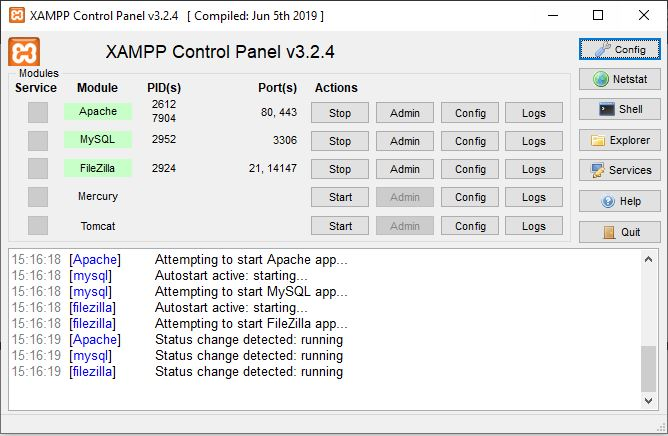
\includegraphics[width=0.7\linewidth]{sezioni/FaseTest/Immagini/xampp.JPG}\\
	\caption{XAMPP Control Panel}
	\label{Fig:xampp}
\end{figure} 